
\chapter{Visi\'{o}n general}

Desde una perspectiva global, para generar un mapa 3D de la condición de erosión de un modelo físico utilizando una cámara RGB-D, es necesario ejecutar las siguientes etapas:
\begin{itemize}

\item Captura del frame RGB-D a partir del sensor (o lectura desde el sistema de archivos si ya hubiese sido grabado).

\item Registración del frame RGB-D. Se alinea el frame a un sistema de coordenadas de referencia (sistema modelo).

\item Eliminación de inconsistencias. La cámara puede relevar puntos sin información de profundidad o con mediciones incorrectas que deben ser filtrados para obtener mapas 3D consistentes. 

\item Conversión del sistema de coordenadas modelo al sistema prototipo. Inicialmente, el conjunto de frames (habiendo sido alineados o no) están en un sistema de coordenadas que tiene su origen en el sensor. Se transforma el sistema de coordenadas y se aplica el cambio de escala correspondiente (propiedad de construcción del modelo físico), a fin de obtener un modelo 3D que representa el mapa digital de elevaciones de la condición de erosión en prototipo.

\end{itemize}

En este trabajo, la etapa de captura y registración se ejecutan incrementalmente hasta obtener un mapa 3D de la escena observada. Una vez finalizada la alineación, se realiza la eliminación de inconsistencias y finalmente se lleva a cabo la conversión a prototipo. En la figura \ref{fig:esquema-general-aplicacion} se ilustra el procedimiento implementado.
En los siguientes capítulos se explica con mayor detalle cada una de las etapas mencionadas.

\begin{figure}[ht]
\centering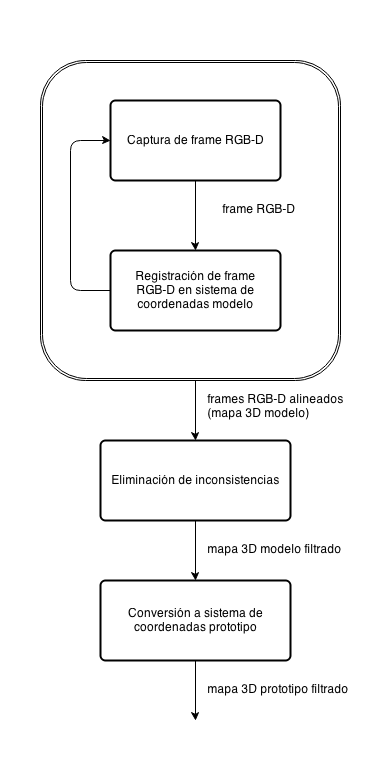
\includegraphics[width=\imsize]
{esquema-general-aplicacion}
\caption[Esquema general para generar mapa 3D en escala prototipo a partir de frames RGB-D.]
{Esquema general para generar mapa 3D en escala prototipo a partir de frames RGB-D.}
\label{fig:esquema-general-aplicacion}
\end{figure}
